\documentclass{report}
\usepackage[margin=1in, paperwidth=8.5in, paperheight=11in]{geometry}
%Math packages%
\usepackage{amsmath}
\usepackage{amsthm}
%Spacing%
\usepackage{setspace}
\onehalfspacing
%Lecture number%
\newcommand{\lectureNum}{3}
%Variables - Date and Course%
\newcommand{\curDate}{January 9, 2017}
\newcommand{\course}{MATH 239}
\newcommand{\instructor}{Peter Nelson (substitute)}
%Defining the example tag%
%\theoremstyle{definition}%
\newtheorem{ex}{Example}[section]
%Setting counter given the lecture number%
\setcounter{chapter}{\lectureNum{}}
%Package for drawing graphs%
\usepackage{tikz}
\usepackage{verbatim}
\usetikzlibrary{arrows}

\begin{document}
%Note title%
\begin{center}
\begin{Large}
\textsc{\course{} | Lecture \lectureNum{}}
\end{Large}
\end{center} 
\noindent \textit{Bartosz Antczak} \hfill
\textit{Instructor: \instructor{}} \hfill
\textit{\curDate{}}
\rule{\textwidth}{0.4pt}

% Actual Notes%
\section{Graph equality}
We define two graphs being equal if their vertex sets and edge sets are the same. But this is very specific and because of this definition, most graphs aren't considered \textit{equal}. For example, consider the two graphs:
%Graph 1%
\begin{center}
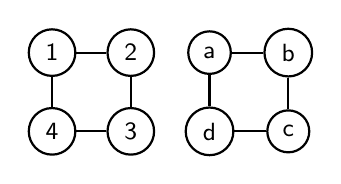
\begin{tikzpicture}[-,auto,node distance=1cm,
                    thick,main node/.style={circle,draw,font=\sffamily\small}]
  %C_4%
  \node[main node] (1) {1};
  \node[main node] (2) [right of=1] {2};
  \node[main node] (3) [below of=2] {3};
  \node[main node] (4) [left of=3] {4};
  %K_{2,2}%
  \node[main node] (5)[right of=2] {a};
  \node[main node] (6)[right of=5] {b};
  \node[main node] (7)[below of=6] {c};
  \node[main node] (8)[left of=7] {d};
  
  \path[every node/.style={font=\sffamily\small}]
    (1) edge node [left] {} (2)
    	edge node [below] {} (4)
    (3) edge node [left] {} (2)
    	edge node[below] {} (4)
    (5) edge node [left] {} (6)
    	edge node [below] {} (8)
    (7) edge node [left] {} (6)
    	edge node[below] {} (8);
\end{tikzpicture}
\end{center}
Even though they look equal, these two graphs are \underline{not} equal, because their sets are not the same ($\{1, 2, 3, 4\} \neq \{a, b, c, d\}$).\\
\noindent For a better definition of graph equality, we look to \textit{isomorphism}.
\subsection{Definition | Isomorphism}
\subsubsection{Recall}
A \textit{bijection} between two sets is a function that is one-to-one \underline{and} onto | in other words, it's a function that maps exactly one item in the first set to exactly one item in the other set; there is a one-to-one correspondence between every item in both sets. For instance, say $\{a, b, c\}$ and $\{1, 2, 3\}$. A possible bijection is $a \rightarrow 1$, $b \rightarrow 2$, $c \rightarrow 3$. \\\\
An \textbf{isomorphism} from graph $G$ to a graph $H$ is a bijection $f$ (or sometimes denoted as $\varphi$) from $V(G)$ to $V(H)$ such that $uv \in E(G)$ if and only if $f(u)f(v)$ is an edge of $H$. Isomorphic graphs have these qualities:
\begin{itemize}
\item the same number of vertices
\item the same number of edges
\item the same number of vertices of any fixed degree $k$
\item the same number of copies of each fixed subgraph $H$
\end{itemize}
All of these properties are \textit{graph invariants}, which are properties that hold for every graph. Graphs that fail any one of these tests must be non-isomorphic.
\subsection{Handshaking theorem}
There are $n$ people in a room, if each person shakes hands with everyone else, how many handshakes are there? This problem leads to an important theorem:\\
Let $G = (V, E)$ be a graph. Then
\begin{equation}
\sum_{v \,\in\, V} \mathrm{deg}(v) = 2 \vert E \vert
\end{equation}
\subsubsection{Proof of handshaking theorem (somewhat formal)}
Count the number of pairs $(v, e)$, where $e$ is an edge of $G$ incident with $v$.\\
Since each vertex $v$ is in deg$(v)$ such pairs, the total number of such pairs is $\displaystyle \sum_{v \,\in\, V} \mathrm{deg}(v)$.\\
Alternatively, since each edge $e$ is in 2 such pairs, the total number of pairs is $2 \vert E \vert$. Thus, $\displaystyle \sum_{v \,\in\, V} \mathrm{deg}(v) = 2 \vert E \vert$

\subsubsection{Corollary 1}
\textit{The number of vertices of odd degree in a graph must be even.}\\
\textbf{Proof}: (contradiction) if there was an odd number of vertices of odd degree, then the sum of their degrees would be odd, which is impossible since the sum of the degrees is equal to $2 \vert E \vert$, which is always even.

\subsubsection{Corollary 2}
\textit{The average degree of the vertices of a graph $G = (V, E)$ is}
\begin{equation}
\frac{2 \vert E \vert}{\vert V \vert}
\end{equation}
\textbf{Proof}: the average degree of the vertices of a graph is defined as
$$\frac{\displaystyle\sum_{v \,\in\, V} \mathrm{deg}(v)}{\vert V \vert} = \frac{2 \vert E \vert}{\vert V \vert}$$
%END%
\end{document}